\documentclass[11pt,a4]{article}
\usepackage[margin=1in]{geometry}
\usepackage{fancyhdr}
\pagestyle{fancy}
\usepackage{lmodern}
\usepackage{lipsum}%% a garbage package //ignore 
\usepackage{hyperref}
\usepackage{graphicx}
\usepackage{enumitem}
\usepackage{xcolor}
\usepackage{listings}
\lstset{basicstyle=\ttfamily,
	showstringspaces=false,
	commentstyle=\color{red},
	keywordstyle=\color{blue}
}
%*****************************************************************************%
\title{\textbf{Assignment 4}}   % Make sure to change the number when necessary
\author{Satyam Kumar \\ ID: 201552062} % Your name and ID
\date{}
\lhead{\textbf{Assignment 4}}     % Assignment #No0101
\rhead{\textbf{201552062}}        % Student ID  
%*****************************************************************************%
\begin{document}
\maketitle
\section*{2. Procedure used to crack the User's password.}
\begin{enumerate}
%\parbox[b]{0.9\textwidth}
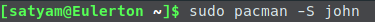
\includegraphics[width=10cm]{install.png}
%\newline
\item Store user's name (anonymous) and encypted value in a text file and save it in a home directory.
\item Run /textit{/usr/sbin/john --text} command. This command creates new hidden file in home direcrtory\\

\includegraphics[width=10cm]{test.png}
\item  To crack password, type the following command with the name of file in which password is stored. \\
/textit{/usr/sbin/john password.txt}\\This may take few minute to few hours, depending upon the speed of processor.\\

\includegraphics[width=10cm]{PW_text.png}
\item The cracked password of the user obtained and it is \textbf{system} as can be seen from the image.\\

\includegraphics[width=10cm]{PW_cracked.png}
\section*{3. Write a Bash script to add the following users (in a batch mode).}
\begin{lstlisting}[language=bash]
#!/bin/bash
USERNAME=$(cat userlist.txt | cut -d: -f1)
echo "$USERNAME"

PWd=$(cat userlist.txt | cut -d: -f2)
echo "$PWd"

UID=$(cat userlist.txt | cut -d: -f3)
echo "$UID"

GID=$(cat userlist.txt | cut -d: -f4)
echo "$GID"

USER_SHELL=$(cat userlist.txt |  cut -d: -f5)
echo "$USER_SHELL"

useradd -m -s "$USER_SHELL" -u "$UID" -g "$GID" "$USERNAME" -p "$PWd"
\end{lstlisting}
\section*{4. Write (1) description (purpose), (2) example(s), and (3) output of following commands
	or command-line switches.}
\subsection*{4.1. w}
w - Show who is logged on and what they are doing.\\
Example(s): w\\
Output: w : displays  information  about the users currently on the machine, and
their processes.\\\\
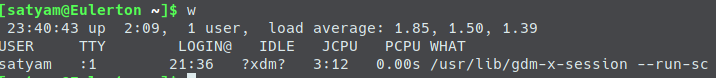
\includegraphics[width=\textwidth]{Q4_1.png}
\subsection*{4.2. id}
id - print real and effective user and group IDs\\
Example(s): id\\
Output: Print user and group information for the specified USER \\\\
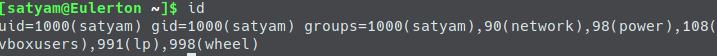
\includegraphics[width=\textwidth]{Q4_2.png}
\subsection*{4.3. id -g}
id -g : print only the effective group ID\\
Example(s): id -g \\
Output: 1000(gid)
%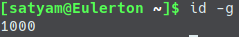
\includegraphics[width=\textwidth]{Q4_3.png}
\subsection*{4.4. id -G}
id -G : print all groups\\
Example(s): id -G \\
Output: 1000 90 98 108 991 998
\subsection*{4.5. id -u}
id -u : print only effective user id\\
Example(s): id -u \\
Output: 1000
\subsection*{4.6. id -n}
id -n :print a name instead of a number, for -ugG\\
Example(s): id - n\\
Output: cannot print only names or real IDs in default format

\subsection*{4.7. id -gn}
id -gn :print a group name\\
Example(s): id - gn\\
Output:  satyam
\subsection*{4.8. id -un}
id -un :print a user name\\
Example(s): id - un\\
Output: satyam
\subsection*{4.9. groups}
groups - display current group names
Example(s): groups\\
Output: satyam
\subsection*{4.10. groups $<$user-name$>$}
groups <user-name> - display current group names
Example(s): groups satyam\\
Output: wheel lp network power vboxusers satyam 

\subsection*{4.11. su}
su - run a command with substitute user and group ID
Example(s): su\\
Output: su allows to run commands with a substitute user and group ID.

\subsection*{4.12. su -}
su - :Start the shell as a login shell with an environment similar to a real login:
Example(s): su -\\
Output: root login
\subsection*{4.13. su $<$user-name$>$}
Example(s): su satyam\\
Output: No root login
\subsection*{4.14. su - $<$user-name$>$}
Example(s): su - satyam\\
Output:Login back to USERS

\subsection*{4.15. chsh}
chsh :  change your login shell\\
Example(s): chsh\\
Output: chsh is used to change your login shell.  If a shell is not given on the command line, chsh prompts for one.

%\subsection*{4.16. chsh -s $<$shell-name/path$>$}
\subsection*{4.17. passwd}
passwd - change user password\\
Example(s): passwd\\
Output: The passwd command changes passwords for user accounts. passwd also changes the
account or associated password validity period.

\subsection*{4.18. passwd -S}
passwd -S Display account status information.\\
Example(s): passwd -S\\
Output:satyam P 07/05/2018 0 99999 7 -1
\subsection*{4.19. passwd -d $<$user-name$>$}
Delete a user's password (make it empty)\\
Example(s): sudo passwd -d satyam\\
Output:password expiry information changed.
\subsection*{4.20. passwd -e $<$user-name$>$}
 Lock the password of the named account.\\
Example(s): passwd -e satyam\\
Output:password expiry information changed.
\subsection*{4.21. passwd -l $<$user-name$>$}
 Lock the password of the named account.\\
Example(s): passwd -l satyam\\
Output:password expiry information changed.
\subsection*{4.22. passwd -n $<$user-name$>$}
Set the minimum number of days between password changes to MIN\_DAYS.\\
Example(s): passwd -n 1  satyam\\
Output:password expiry information changed.
\subsection*{4.23. passwd -u $<$user-name$>$}
unlock the password of the named account\\
Example(s): passwd -u satyam\\
Output:password expiry information changed.
\subsection*{4.24. passwd -w $<$user-name$>$}
Set expiration warning days to WARN\_DAYS\\
Example(s): passwd --warndays 3 satyam\\
Output:password expiry information changed.
\subsection*{4.25. passwd -x $<$user-name$>$}
Set expiration warning days to MAX\_DAYS\\
Example(s): passwd --warndays 3 satyam\\
Output:password expiry information changed.
\subsection*{4.26. chage -l $<$user-name$>$}
Change user password expiry information\\
Example(s): chage -l satyam\\
Output:\\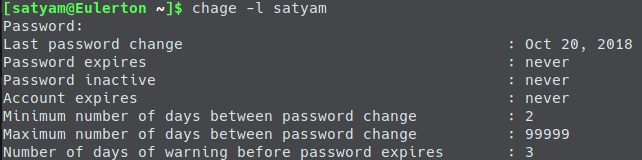
\includegraphics[width=\textwidth]{Q4_26.png}
\subsection*{4.27. chage -d $<$value$>$ $<$user-name$>$}
 set date of last password change to LAST\_DAY\\
 Example(s):chage -d 30000 satyam\\
 Output: Last password change : Feb 20, 2052
 
\subsection*{4.28. chage -E $<$value$>$ $<$user-name$>$}
set account expiration date to EXPIRE\_DATE
Example(s): chage -E 30 satyam\\
Output: Account expires	: Jan 31, 1970
\subsection*{4.29. chage -m $<$value$>$ $<$user-name$>$}
set minimum number of days before password change to MIN\_DAYS\\
Example(s): chage -m 1 satyam\\
Output: Minimum number of days between password change: 1
\subsection*{4.30. chage -M $<$value$>$ $<$user-name$>$}
set maximum number of days before password change to MAX\_DAYS\\
Example(s): chage -m 28 satyam\\
Output: Maximum number of days between password change: 28
\subsection*{4.31. gpasswd $<$group-name$>$}
gpasswd - administer /etc/group and /etc/gshadow\\
Example(s): gpasswd satyam\\
Output: Ask to change group password
\subsection*{4.32. gpasswd -a $<$user-name$>$ $<$group-name$>$}
Add the user to the named group.\\
Example(s): gpasswd -a satyam som\\
Output:Set password for new user Som
\subsection*{4.33. gpasswd -d $<$user-name$>$ $<$group-name$>$}
Delete the user to the named group\\
Example(s): gpasswd -d steve sysadmin
Output: Removing user steve from group sysadmin

\subsection*{4.34. gpasswd -r $<$group-name$>$}
Remove the GROUP's password\\
Example(s): gpasswd -r vinay\\
Output:Password of vinay is removed.
\subsection*{4.35. gpasswd -M $<$user-name1,user-name2,...$>$ $<$group-name$>$}
gpasswd -M : set the list of members of GROUP\\
Example(s): gpasswd -M bill steve sysadmin\\
Output:sysadmin:x:1001:bill,steve

\subsection*{4.36. adduser $<$user-name$>$}
Example(s): adduser vinay\\
Output: No output
\subsection*{4.37. useradd $<$user-name$>$}
useradd - create a new user or update default new user information\\
Example(s): useradd vinay\\
Output:User Vinay added.
\subsection*{4.38. useradd -d $<$home-dir$>$ $<$user-name$>$}
 The new user is created using HOME\_DIR as the value for the
user's login directory.\\
Example(s): useradd -d /home/vinayak vinayak\\
Output:User Vinayak added in /home/vinayak from /home/satyam
\subsection*{4.39. useradd -u $<$UID$>$ $<$user-name$>$}
useradd -u:The numerical value of the user's ID.\\
Example(s):useradd -u 1234 vinayak\\
Output:User Vinayak with userid 1234\\
To check user has been added or not : getent passwd $|$ grep  vinayak\\
\textit{vinayak:x:1234:1234::/home/vinayak:/bin/bash}
\subsection*{4.40. useradd -g $<$GID$>$ $<$user-name$>$}
 useradd -g :Sets the initial, or primary, group.\\
 Example(s):useradd -G 123 vinayak\\
 Output:User Vinayak with groupid 1234 is added
\subsection*{4.41. useradd -G $<$group1/GID1,group2/GID2,...$>$ $<$user-name$>$}
useradd -G: Sets the supplementary, or additional, groups.\\
 Example(s):useradd -G steve,bill vinay2\\
Output: steve:x:1002:vinay2\\
bill:x:1003:vinay2



\subsection*{4.42. useradd -s $<$login-shell$>$ $<$user-name$>$}
The name of the user's login shell.\\
 Example(s):useradd -s /bin/sh vinay\\
Output:vinay1:x:1235:1235::/home/vinay1:/bin/sh
\subsection*{4.43. usermod $<$user-name$>$}
 usermod - modify a user account.\\
Example(s):usermod vinay\\
Output:
\subsection*{4.44. usermod -d $<$home-dir$>$ $<$user-name$>$}
usermod -d : new home directory for the user account\\
Example(s):usermod -d /home/vinay1 vinay\\
Output: User vinay's home directory is modified to /home/vinay1

\subsection*{4.45. usermod -g $<$group/GID$>$ $<$user-name$>$}
usermod -g: Changes group of user to another Group with other being  new primary group\\
Example(s):usermod -g vinay vinay1\\
Output:vinay1:x:1235:

\subsection*{4.46. usermod -G $<$group1/GID1,group2/GID2,...$>$ $<$user-name$>$}
usermod -G : new list of supplementary GROUPS\\
Example(s):usermod -G vinay,vinay1 steve
\\
Output:vinay1:x:1235:steve\\vinay:x:1004:steve

\subsection*{4.47. usermod -l $<$new-user-name$>$ $<$user-name$>$}
usermod - l:new value of the login name\\
Example(s):usermod -l vinay2 vinayak
\\
Output:getent passwd | grep  vinay2\\
vinay2:x:1234:1234::/home/vinayak:/bin/bash

\subsection*{4.48. usermod -L $<$user-name$>$}
usermod -L :Lock the user account \\
Example(s):usermod -L vinay2\\
Output:getent passwd | grep  vinay2\\
vinay2:x:1234:1234::/home/vinayak:/bin/bash

\subsection*{4.49. usermod -U $<$user-name$>$}
usermod -U :Unlock the user account \\
Example(s):usermod -U vinay2\\
Output: Unlocking the user's password would result in a passwordless account.

\subsection*{4.50. deluser $<$username$>$}
No such command found.
\subsection*{4.51. userdel $<$username$>$}
userdel - delete a user account and related files\\
Example(s):userdel vinay2\\
Output: No user vinay2 found.

\subsection*{4.52. addgroup $<$group-name$>$}
No manual entry for addgroup\\
Example(s):addgroup  vinay2
\subsection*{4.53. groupadd -g $<$GID$>$ $<$group-name$>$}
groupadd - create a new group\\
Example(s):groupadd sv\\
Output:sv:x:1236:

\subsection*{4.54. groupmod $<$group-name$>$}
groupmod - modify a group definition on the system\\
Example(s):groupmod sv\\
Output:sv:x:1236:
\subsection*{4.55. groupmod -g $<$new-GID$>$ $<$group-name$>$}
groupmod -g: The group ID of the given GROUP will be changed to GID.\\
Example(s):groupmod -g 1007 sv\\
Output:sv:x:1007:

\subsection*{4.56. groupmod -n $<$new-group-name$>$ $<$group-name$>$}
 groupmod -n: The name of the group will be changed from GROUP to NEW\_GROUP name.\\
 Example(s):groupmod -n sysadmin1 sv\\
 Output:sysadmin1:x:1007:

\subsection*{4.57. delgroup $<$group-name$>$}
No manual page for delgroup
\subsection*{4.58. groupdel $<$group-name$>$}
 groupdel - delete a group\\
Example(s):groupdel sysadmin1\\
Output:No group sysadmin1 found.

\subsection*{4.59. finger $<$user-name$>$}
No manual entry for finger
\subsection*{4.60. chfn $<$user-name$>$}
  chfn -        chfn  is  used  to  change  your  finger  information.   This  information  is stored in the
  /etc/passwd file, and is displayed by the finger program. \\
  Example(s):chfn steve\\
  Output:\\
  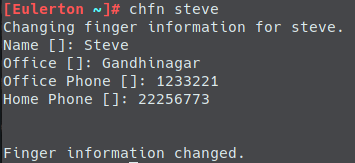
\includegraphics[width=10cm]{Q4_60.png}
  

\end{enumerate}

\section*{5. Write the following answers. Replace $<$your-name$>$ with your real name.}
\subsection*{5.1. Add three users,$<$your-name$>$, Bill, Steve. Users $<$your-name$>$ and Bill are
	also a part of the group, “SysAdmin”. In addition, disable the user Steve’s shell
	access.}
groupadd sysadmin\\
useradd bill
useradd -s /usr/sbin/nologin steve\\
gpasswd -a satyam sysadmin\\
gpasswd -a bill sysadmin\\
gpasswd -a steve sysadmin

%\subsection*{	5.1. Add three users,$<$your-name$>$, Bill, Steve. Users $<$your-name$>$ and Bill are also a part of the group, “SysAdmin”. In addition, disable the user Steve’s shell}	
	\subsection*{5.2 Automatically add a file $<$your-name>.txt to all new user’s account (or home directory).}
		
		\subsection*{5.3 Add a user account, <your-name>, and set the account expiry date on 30-Nov-2018.}
		usermod -e 2018-11-30 satyam\\
	   chage -l satyam
		\subsection*{	5.4. Create a user named Mark, where the user ID is 123 and password is Mark123.}
useradd -u 123 mark\\
 passwd Mark
 \subsection*{5.6. Change the user $<$your-name$>$’s group to “Guest”.}
 groupmod -n guest satyam
\subsection*{5.7. Change the password of your root user account}
  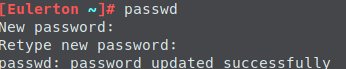
\includegraphics[width=10cm]{Q57.png}
\subsection*{5.8. Change the default “bash shell” of your user account. The change should be permanent.}
chsh -s /bin/bash
%\section{Installation of CentOS in Virtualbox}
%\begin{enumerate}
%\parbox[b]{0.9\textwidth}{%
%	\item 	Open Virtual Box and select New menu from Machine icon present in the toolbar icon. Name of the Virtual Machine is given anything that you think of. I have given the name CentOs 7. Choose Linux as Operating System Type and Red Hat(64-bit) as the version.  
%}\vfill\includegraphics[width=10cm]{CentOS.png}
%\newline
% 	
%\parbox[b]{0.9\textwidth}{%
%	\item  Click on Next and choose the amount of RAM memory for VM.The suggested amount, which is 1024 MB(1GB) is been selected. It can be increased, based on requirements.
%}\vfill\includegraphics[width=10cm]{RAM_Alloc.png}
%\newline
%
%\parbox[b]{0.9\textwidth}{%
%	\item  The next prompt will ask you to add a virtual hard disk. Go ahead and select Create a virtual hard disk now which should be the default.
%}\vfill\includegraphics[width=10cm]{Harddisk_virtualization.png}
%\newline
%
%\parbox[b]{0.9\textwidth}{%
%\item On clicking next, type of VM hard disk is selected. Default is VirtualBox disk image(VDI).
%}\vfill\includegraphics[width=10cm]{VB2.png}
%\newline
%
%\parbox[b]{0.9\textwidth}{%
% \item Next prompt ask you to choose dynamic or fixed storage. Select dynamic, which is default. Fixed size memory creates issues later on.
%}\vfill\includegraphics[width=10cm]{CentOs3.png}
%\newline
%
%\parbox[b]{0.9\textwidth}{%
% \item Next prompt is to allot the amount of hard disk space for the Virtual Machine. 8.00GB is the default value.It is recommended to have atleast  15GB. I have alloted 30GB of hard disk space to VM  Go ahead and press the Create button to finish up this part of the process.
%}\vfill\includegraphics[width=10cm]{File_loc.png}
%\newline
%
%\parbox[b]{0.9\textwidth}{%
%	\item Virtual Machine will reappear. In that window, one will see the name of the Operating System. Operating System will be powered off. 
%}\vfill\includegraphics[width=10cm]{Poweroff.png}
%\newline \\
%\begin{minipage}[b]{0.9\textwidth}{%
%\item Install \href{centos.org}{CentOS}. Click on Get Everything tab and download the ISO file from your country's nearest mirror(or server) and save it in local directory.
%}\vfill\includegraphics[width=10cm]{Centos_mirror.png}
%\end{minipage}
%\newline 
%\begin{minipage}[b]{0.9\textwidth}{%
%	\item Click on Settings icon, present in the toolbar. Go to storage tab and click on  Controller:IDE.New column on right appears.On clicking on Optical drive, select the ISO file, which has been downloaded and stored in local directory. 
%}\vfill	\includegraphics[width=10cm]{Centos_settings.png}
%\end{minipage}
%\newline \\
%\begin{minipage}[b]{0.9\textwidth}{%
%		\item After ISO is loaded, select System tab and also select Network as Boot Option. After that click on Start button, present in Toolbar.
%	}\vfill	\includegraphics[width=10cm]{Settings2.png}
%\end{minipage}
%\newline 
%\begin{minipage}[b]{0.9\textwidth}{%
%	\item Install process begins by asking you to select the language of your preference. Once you have choosed language, click on  Continue to move to next tab, present in right-bottom corner.\\
%}\vfill	\includegraphics[width=10cm]{language.png}
%\end{minipage}
%\newline
%\begin{minipage}[b]{0.9\textwidth}{%
%		\item Select Date and Time \\
%	}\vfill	\includegraphics[width=10cm]{Installation_destination.png}
%\end{minipage}
%\newline
%\begin{minipage}[b]{0.9\textwidth}{%
%	\item Select Time zone you are in and press Done\\
%}\vfill	\includegraphics[width=10cm]{datetime.png}
%\end{minipage}
%\newline
%\begin{minipage}[b]{0.9\textwidth}{%
%		\item Select the hostname give hostname and Select the network card and press configure button\\
%	}\vfill	\includegraphics[width=10cm]{Ethernet.png}
%\end{minipage}
%\newline
%
%\begin{minipage}[b]{0.9\textwidth}{%
%	\item In system menu, select the installation destionation, and keep the default partioning ie automatic configuration partioning.Click on Begin Installation.\\
%}\vfill\includegraphics[width=10cm]{installation_destination.png}
%\end{minipage}
%\newline
%
%\begin{minipage}[b]{0.9\textwidth}{%
%		\item The install will begin, but there are still two more steps we need to take. The next window will give us the opportunity to set the root password and to add an additional account.\\
%	}\vfill\includegraphics[width=10cm]{user_creation.png}
%\end{minipage}
%
%\begin{minipage}[b]{0.9\textwidth}{%
%		\item Select Root Password and create a new password for the root account.\\
%	}\vfill\includegraphics[width=10cm]{root_pwd.png}
%\end{minipage}
%
%\begin{minipage}[b]{0.9\textwidth}{%
%		\item Create New User. Go ahead and make the user an administrator.\\
%	}\vfill\includegraphics[width=10cm]{user_creation1.png}
%\end{minipage}
%\newline
%\item Once this is finished, the bottom of prompt will display a message that Installation is finished. Click on Restart.
%\newline \\
%
%\begin{minipage}[b]{0.9\textwidth}{%
%		\item As the system restarts, new screen appears,similar to GRUB. Select the first option.\\
%	}\vfill\includegraphics[width=10cm]{Boot.png}
%\end{minipage}
%\newline
%\begin{minipage}[b]{0.9\textwidth}{%
%		\item Once the system reboots,you will get a Initial Setup screen. Click on License Information.\\
%	}\vfill\includegraphics[width=10cm]{Setup_reboot.png}
%\end{minipage}
%\newline
%\begin{minipage}[b]{0.9\textwidth}{%
%		\item After clicking on License Information, select the accept agreement.\\
%	}\vfill\includegraphics[width=10cm]{License_agreement.png}
%\end{minipage}
%\newline
%\begin{minipage}[b]{0.9\textwidth}{%
%		\item Once everything is done, Login GUI will appear with your name that you have typed during creation.\\
%	}\vfill\includegraphics[width=10cm]{Login_GUI.png}
%\end{minipage}
%\newline
%\begin{minipage}[b]{0.9\textwidth}{%
%		\item After entering your Password. New Popup window will appear for further confirmation of Language and Keyboard Layout.\\
%	}\vfill\includegraphics[width=10cm]{GNOME_Setup.png}\\\\\includegraphics[width=10cm]{Keyboard.png}
%\end{minipage}
%\newline
%Click on Start using CentOs 7.
%%\item Check for ssh in Virtual Machine. After this you need to install GUI through terminal.
%%Following commands are used for installing GUI
%%\begin{enumerate}[label=\roman*]
%%	\item Console with network enable - \\ \textit{systemctl get-default}
%%	\item Start GUI -\\ \textit{systemctl isolate graphical.target}
%%	\item  If we perform a reboot we will not be presented with the GUI. To do this, we must first set the graphical target to become the default -\\ \textit{systemctl set-default graphical.target}
%%\end{enumerate}
%%After completion of steps related to installation of GUI, reboot the system.
%\end{enumerate}
%\section{Known Command (Q5)}
%\begin{itemize}
%	\item ls(Listing): ls -la, ls -a
%	\\Functionality : To list all files present in a directory.
%	\item cat filename, cat > filename
%	\\Functionality To view content of multiple files and also to display content in the screen. To create file using cat.
%	\item touch filename
%	\\Functionality To create new empty file.
%	\item mv file1 file2
%	\\Functionality To move files or directory from one location (source) to another location (destination)
%	\item rm(Remove): rm file1, rm -r dir
%	\\Functionality To remove files or directory if not required.
%	\item cp(Copy): cp src destination
%	\\Functionality To copy files from source to directory.
%	\item ip addr
%	\\Functionality To find ip address of networking devices connected with computer or laptop.
%	\item lspci
%		\\Functionality To list all hardware devices(PCI devices)
%		\item pwd
%		\\Functionality: To print the current working directory.
%\end{itemize}

\end{document}